\documentclass[12pt,twoside, a4paper, twocolumn]{article}
\usepackage[utf8]{inputenc}
\usepackage[brazil]{babel}
\usepackage[margin = 0.5in]{geometry}
\usepackage{amsmath}
\usepackage{amsthm}
\usepackage{amssymb}
\usepackage{amsthm}
\usepackage{setspace}
\usepackage[americanvoltages,fulldiodes,siunitx]{circuitikz}
\usepackage{lipsum}
\usepackage{pgfplots}
\usepackage{ifthen}
\usepackage{adjustbox}
\usepackage[section]{placeins}
\usepackage{hyperref}
\usepackage{graphicx}
\usepackage{amsmath}
\usepackage{amsthm}
\usepackage{amssymb}
\usepackage{amsthm}
\usepackage{setspace}
\usepackage[americanvoltages,fulldiodes,siunitx]{circuitikz}
\usepackage{lipsum}
\usepackage{pgfplots}
\usepackage{ifthen}
\usepackage{adjustbox}
\usepackage[section]{placeins}
\usepackage{hyperref}
\usepackage{graphicx}
\usepackage{adjustbox}
 
\pgfplotsset{compat=newest}
 
\graphicspath{ {./images/} }
 
%  #1 color - optional #2 x_0 #3 y_0 #4 x_f #5 y_f #6 name - optional  #7 true if adding lines to axis
 
\newcommand{\drawvector} [9] [color=cyan] {
   \draw[line width=1.5pt,#1,-stealth](axis cs: #2, #3)--(axis cs: #4, #5) node[anchor=south west]{$#6$};
 
  
 
\ifthenelse{\equal{#7}{true}}{
   \draw[line width=1pt,#1, dashed](axis cs: #4, #5)--(axis cs: #4, 0) node[anchor= north west]{$#8$};
   \draw[line width=1pt,#1, dashed](axis cs: #4, #5)--(axis cs: 0, #5) node[anchor=south east]{$#9$};
   }
   {}
}
 
\newcommand\deriv[2]{\frac{\mathrm d #1}{\mathrm d #2}}
 
 
\title{Segundo Relatório de Medidas Eletromagneticas}
\author{Gabriel Soares \\ Henrique da Silva}
\date{\today}
\pgfplotsset{width = 10cm, compat = 1.9}
 
 
\begin{document}
\maketitle
\pagenumbering{gobble}
\newpage
%pagenumbering{roman}
\tableofcontents
\newpage



\section{Introdução}


\subparagraph*{Neste relatório, vamos medir os valores de resistencia $\varOmega$ e capacitancia $F$ de resistores e capacitores, e calcularemos alguns de seus parametros estatisticos.}

\subparagraph*{Todos arquivos utilizados para criar este relatorio, e o relatorio em si estão em:  \url{https://github.com/Shapis/ufpe_ee/tree/main/5th semester/lab circuitos}}




\subsection{Analise preliminar}
\subparagraph*{}


\subparagraph*{Utilizaremos um multimetro para medir as propriedades de alguns componentes.}

\subparagraph*{Faremos $20$ medicoes em cada componente, e calcularemos a media, desvio padrao, tendencia, e correcao de cada um deles.}

\subparagraph*{Apos isto discutiremos os nossos achados.}

\section{Resultados esperados}

\subsection{Resistor}

\subparagraph*{Esperamos resultados consistentes entre as medidas, porem, tambem esperamos que a resistencia seja diferente da resistencia de fabrica.}

\subparagraph*{Isto ocorrera por desgaste dos componentes devido a seu uso de laboratorio, e tambem pela qualidade dos componentes.}

\subparagraph*{Muito provavelmente estamos fora dos padroes de confiabilidades de fabrica. Mas precisariamos ver o datasheet dos resistores em especifico para confirmar isto.}

\subsection{Capacitor}

\subparagraph*{Tudo que falamos a cima se aplica aos capacitores, mas com dois diferenciais.}

\subparagraph*{O primeiro eh que estes sao mais sensiveis ao uso, logo esperaremos discrepancias maiores entre os valores de fabrica e os de fato.}

\subparagraph*{E tambem que durante as medidas, os carregaremos e os descarregaremos, que implicara tambem em um erro sistematico adicional.}


\section{Medicoes no Laboratorio}

\subparagraph*{Utilizando um multimetro, mediremos resistencias de resistores, e capacitancias de capacitores.}

\subparagraph*{Para reduzir erros sistematicos, os encaixaremos todos componentes em um protoboard.}

\subparagraph*{E antes de fazer as medidas dos capacitores, vamos criar um circuito com um capacitor e um resistor em serie para descarregalos. Apos alguns segundos com este circuito formado, desconectaremos o circuito e faremos a medicao de fato.}

\subsection{Tabela de medicoes}

\subsubsection{Resistores}

\subparagraph*{Mediremos tres resistores, com valores de fabrica respectivamente de: $R_1 = 10k \varOmega$, $R_2 = 22k \varOmega$, $R_3 = 15k \varOmega$.}
\begin{center}
    \begin{tabular}{ |c|c|c| }
        \hline
        $R_1$ $10k\varOmega$ & $R_2$ $22k\varOmega$ & $R_3$ $15k\varOmega$ \\
        10037 $\varOmega$    & 21932 $\varOmega$    & 14848 $\varOmega$    \\
        10037 $\varOmega$    & 21932 $\varOmega$    & 14849 $\varOmega$    \\
        10038 $\varOmega$    & 21932 $\varOmega$    & 14850 $\varOmega$    \\
        10038 $\varOmega$    & 21932 $\varOmega$    & 14849 $\varOmega$    \\
        10038 $\varOmega$    & 21932 $\varOmega$    & 14850 $\varOmega$    \\
        10037 $\varOmega$    & 21933 $\varOmega$    & 14849 $\varOmega$    \\
        10037 $\varOmega$    & 21933 $\varOmega$    & 14849 $\varOmega$    \\
        10037 $\varOmega$    & 21931 $\varOmega$    & 14850 $\varOmega$    \\
        10037 $\varOmega$    & 21931 $\varOmega$    & 14850 $\varOmega$    \\
        10037 $\varOmega$    & 21930 $\varOmega$    & 14848 $\varOmega$    \\
        10036 $\varOmega$    & 21932 $\varOmega$    & 14849 $\varOmega$    \\
        10037 $\varOmega$    & 21932 $\varOmega$    & 14849 $\varOmega$    \\
        10037 $\varOmega$    & 21932 $\varOmega$    & 14849 $\varOmega$    \\
        10037 $\varOmega$    & 21932 $\varOmega$    & 14849 $\varOmega$    \\
        10038 $\varOmega$    & 21934 $\varOmega$    & 14849 $\varOmega$    \\
        10036 $\varOmega$    & 21934 $\varOmega$    & 14850 $\varOmega$    \\
        10036 $\varOmega$    & 21934 $\varOmega$    & 14849 $\varOmega$    \\
        10037 $\varOmega$    & 21933 $\varOmega$    & 14849 $\varOmega$    \\
        10036 $\varOmega$    & 21934 $\varOmega$    & 14849 $\varOmega$    \\
        10036 $\varOmega$    & 21932 $\varOmega$    & 14848 $\varOmega$    \\

        \hline
    \end{tabular}
\end{center}

\begin{center}
    \begin{tabular}{ |c|c|c|c| }
        \hline
        $R_1$ $10k\varOmega$ & $R_2$ $22k\varOmega$ & $R_3$ $15k\varOmega$ & \\
        10037                & 21932                & 14848                  \\
        10037                & 21932                & 14849                  \\
        10038                & 21932                & 14850                  \\
        10038                & 21932                & 14849                  \\
        10038                & 21932                & 14850                  \\
        10037                & 21933                & 14849                  \\
        10037                & 21933                & 14849                  \\
        10037                & 21931                & 14850                  \\
        10037                & 21931                & 14850                  \\
        10037                & 21930                & 14848                  \\
        10036                & 21932                & 14849                  \\
        10037                & 21932                & 14849                  \\
        10037                & 21932                & 14849                  \\
        10037                & 21932                & 14849                  \\
        10038                & 21934                & 14849                  \\
        10036                & 21934                & 14850                  \\
        10036                & 21934                & 14849                  \\
        10037                & 21933                & 14849                  \\
        10036                & 21934                & 14849                  \\
        10036                & 21932                & 14848                  \\

        \hline
    \end{tabular}
\end{center}

\subsection{Graficos dos dados}

\subsubsection{Erro absoluto por frequencia}

% \begin{adjustbox}{scale=0.30}
%     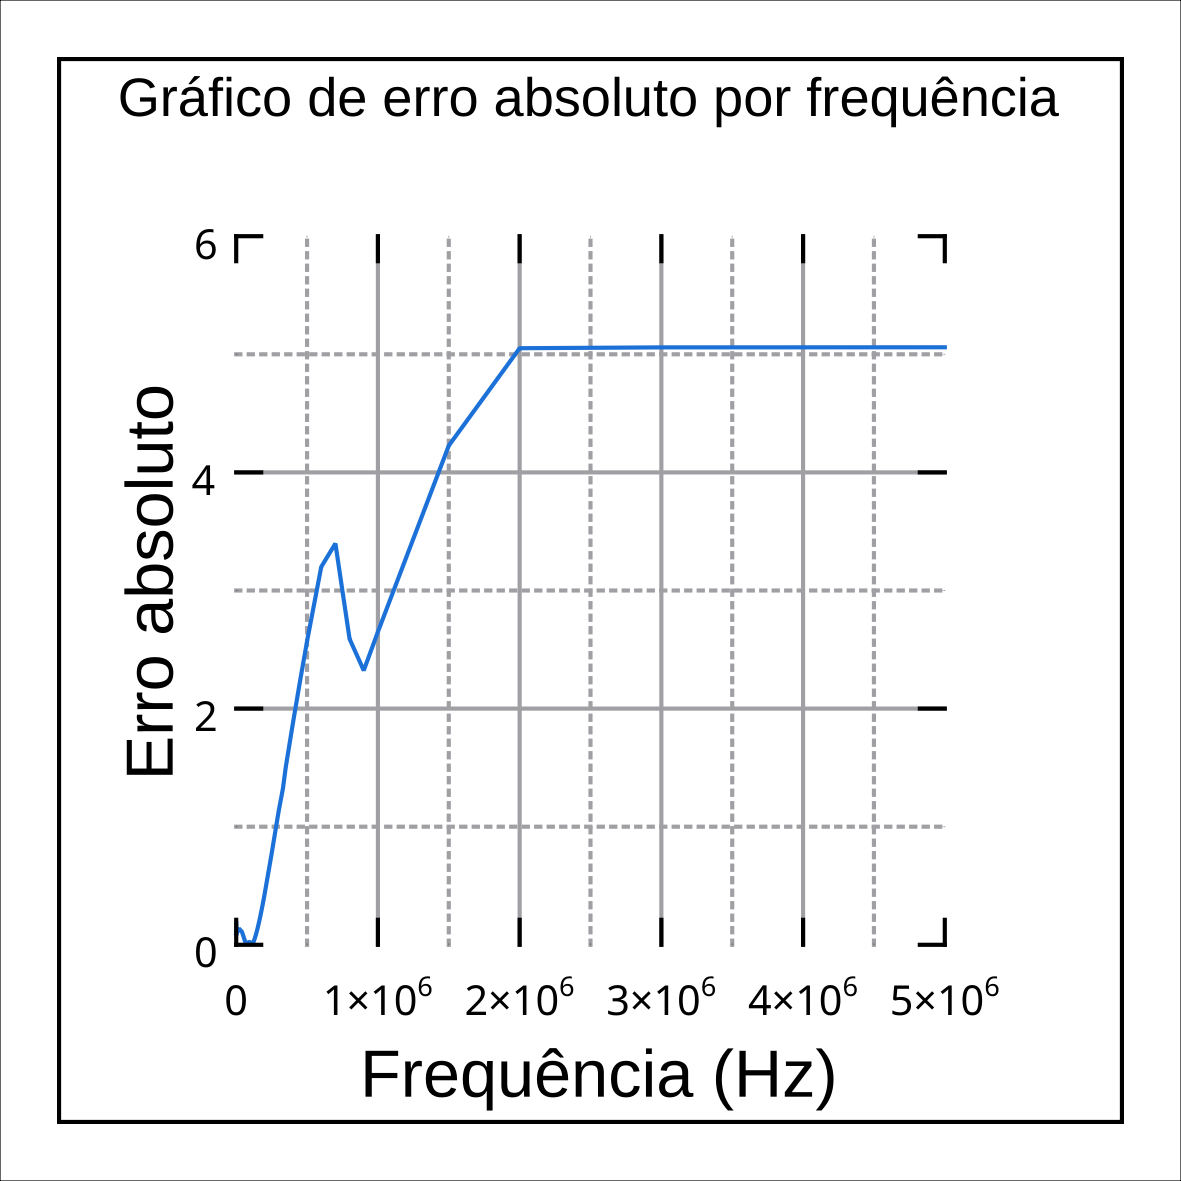
\includegraphics{Grafico1.png}
% \end{adjustbox}

% \subsubsection{Erro percentual por frequencia}

% \begin{adjustbox}{scale=0.30}
%     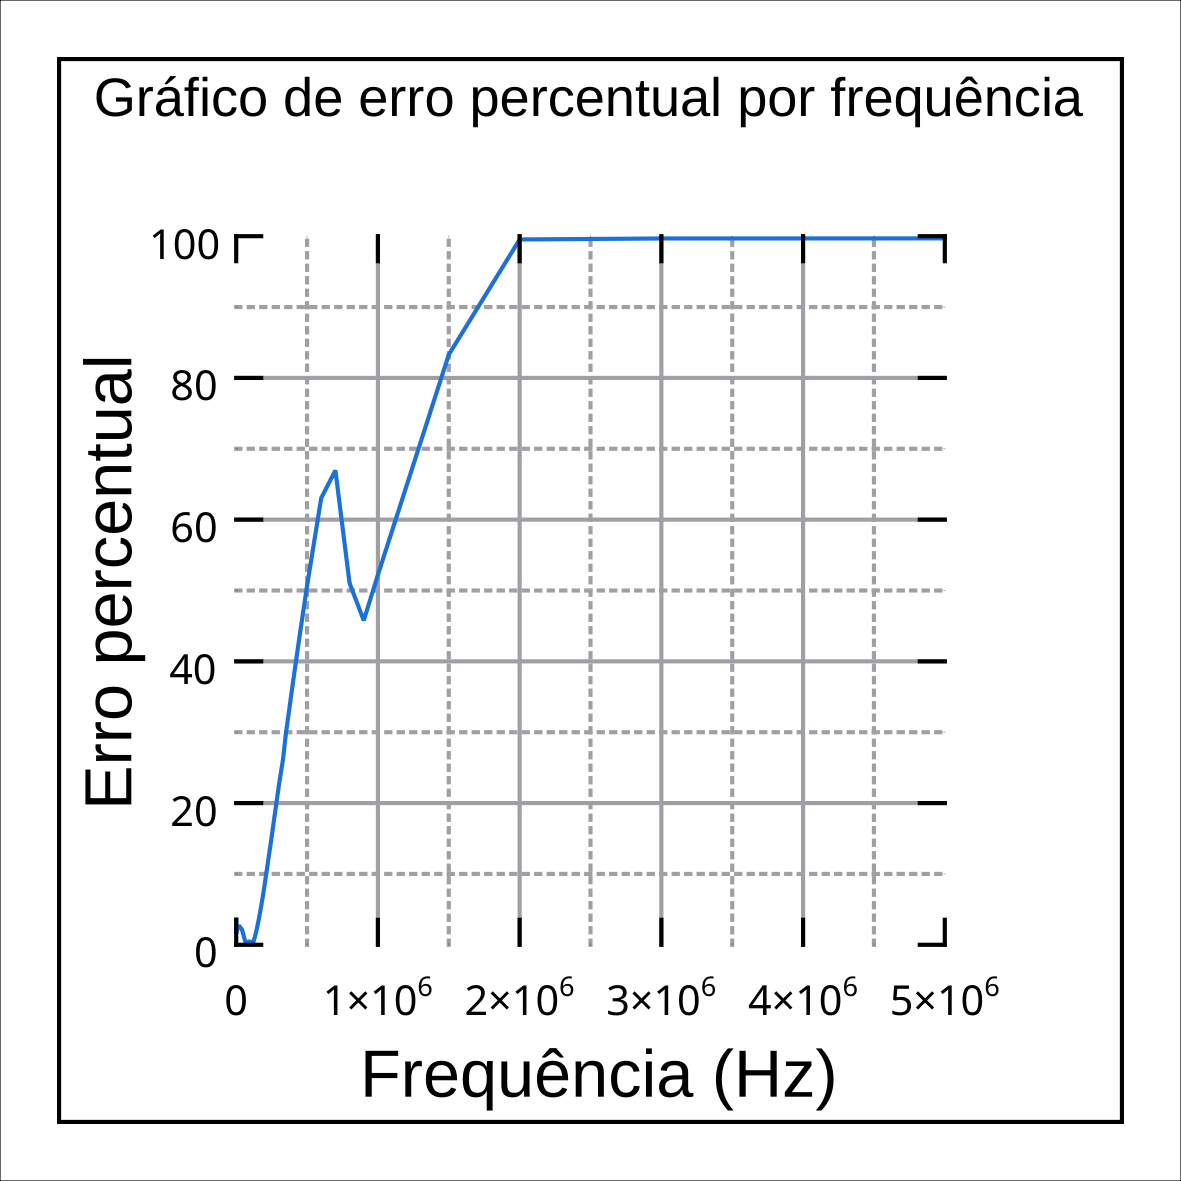
\includegraphics{Grafico2.png}
% \end{adjustbox}

\subsection{Analise da onda dente de serra}

\subparagraph*{Quando analisamos este tipo de onda vimos erros distribuidos ao longo de toda banda de testes.}

\subparagraph*{Isto ocorreu por que a funcao dente de serra pode ser decomposta em senoides, e estas multiplas senoides, obedecerem o erro de acordo com os graficos acima na secao \emph{3.2}.}


\subparagraph*{Logo as senoides decompostas de alta frequencia e baixa nos deram um certo erro consideravel, porem distribuido em toda banda  de testes.}

\newpage
\section{Conclusoes}

\subparagraph*{Vemos que o multimetro tem bastante confianca em uma faixa intermediaria, mas fora desta a confianca eh reduzida significantemente.}

\subparagraph*{Precisamos levar em consideracao tambem o formato da onda de entrada e sua decomposicao por serie de Fourier.}

\subparagraph*{Outro ponto que nao abordamos nesta pratica foi o aspecto da calibracao do multimetro. Esta pode afetar tanto a banda de frequencia de confianca quanto a confianca em todos pontos da banda.}


\end{document}